\documentclass[10pt,preprint]{aastex}
\usepackage{amsmath}
\usepackage{breqn}
\usepackage{cite,natbib}
\usepackage{epsfig}
\usepackage{cases}
\usepackage[section]{placeins}
\usepackage{graphicx, subfigure}

\newcommand{\logg}{log \emph{g}~}
\newcommand{\teff}{$T_{eff}~$}
\newcommand{\prot}{$P_{rot}~$}
\newcommand{\ah}{$\hat{A}_n$}
\newcommand{\ph}{$\hat{P}_n$}
\newcommand{\ch}{$\hat{C}_n$}
\newcommand{\gh}{$\hat{G}_n$}
\newcommand{\yh}{$\hat{Y}_n$}
\newcommand{\teffh}{$\hat{T}_n$}
\newcommand{\dd}{\ensuremath{\,\mathrm{d}}}

\begin{document}

\title{Calibrating Gyrochronology using Kepler Asteroseismic targets}

\author{Ruth Angus$^1$, Suzanne Aigrain$^1$, Amy McQuillan$^2$, Daniel Foreman-Mackey$^3$,  William, J. Chaplin$^4$, Tsevi Maseh$^2$}
\affil{$^1$Department of Physics, University of Oxford, OX1 3RH, UK}
\affil{$^2$School of Physics and Astronomy, Raymond and Beverly Sackler, Faculty of Exact Sciences, Tel Aviv University, 69978, Tel Aviv, Israel}
\affil{$^3$Centre for Cosmology and Particle Physics, New York University, New York, NY, USA}
\affil{$^4$School of Physics and Astronomy, University of Birmingham, Edgbaston, Birmingham, B15 2TT, UK}

\section{Abstract}
\label{abs}

Measuring ages for intermediate and low-mass stars on the main
sequence is challenging, but important for a wide range of studies,
from Galactic dynamics to stellar and planetary evolution.
Among the available methods, gyrochronology is a powerful one, because it requires knowledge of only the star�s mass (or colour) and its rotation period.
However, it is not well calibrated at late ages, and suffers from large uncertainties.
Asteroseismology provides relatively precise age measurements for some of the brightest stars observed by Kepler.
We measured the photometric rotation periods of 144 stars with asteroseismic age in order to calibrate the gyrochronology relation and improve upon current methods of measuring the ages of MS field stars.
We use advanced statistical methods to model the relationship between rotation period, age, and mass (or colour or effective temperature) while accounting for measurement uncertainties in all three quantities.
Our sample includes both main sequence stars and subgiants, and straddles the Kraft break (only main sequence stars cooler than the Kraft break are expected to follow gyrochronology relations); and this must be taken into account when modelling the data.
Once our method is applied to the extended sample of published rotation periods for stars with reliable mass and age estimates, it should enable us to estimate ages for any star with a measured period and mass (or temperature), along with associated uncertainties that reflect both measurement errors and the intrinsic scatter in the gyrochronology relations.

\section{Introduction}
\label{intro}

Stellar ages are notoriously difficult to measure for main sequence (MS) stars.
% Chromospheric activity is often used as an age indicator, as well as lithium depletion, but the evolution of these properties on the main-sequence is poorly understood, plus, high resolution spectra are required to measure either of these properties.
Isochrone placement is one of the most commonly used dating methods for field stars, however it is model-dependent and imprecise, often producing uncertainties of order 100\% or more.
Cluster ages measured by fitting isochrones to an ensemble of coeval stars can have uncertainties as low as 10\% \citep{Soderblom_2010}.
Unfortunately, because the majority of nearby clusters are young, there is a significant deficit of precisely measured ages for old stars and for this reason the current gyrochronology relations are poorly calibrated at late ages.
Photometric rotation periods of stars in the older Kepler clusters will provide excellent anchors for gyrochronology.
The Kepler cluster study \citep{Meibom2011} aims to measure rotation periods for stars in all four open clusters in the Kepler field of view.
The two younger clusters: NGC 6866 (0.5 Gyr) and NGC 6811 (1 Gyr) have been completed, however, the older clusters: NGC 6819 (2.5 Gyr) and NGC 6791 (9 Gyr) are more difficult targets.
Identifying cluster members is tricky since the field is crowded and Kepler pixels are large.
% How many pixels do the clusters cover?
The gyrochronology relations of \citet{Mamajek_2008} were calibrated using activity indicators in young cluster stars and a small number of field stars.
Chromospheric activity, usually measured from the strength of emission in the centers of the broad Ca II H \& K emission lines $R'_{HK}$, is driven by the magnetic dynamo and therefore correlated with rotation (Kraft 1967; Noyes et al. 1984; Montesinos et al. 2001).
The evolution of stellar activity is still poorly understood, especially for older stars and whilst the \citet{Mamajek_2008} relation improves upon the age-colour dependence of the \citet{Barnes_2007} relation, it remains poorly calibrated at late ages.
No existing gyrochronology models correctly describe the spin-down behaviour of stars for all masses and at all ages.

\subsection{Angular momentum loss in Main Sequence stars}
Stars lose angular momentum over their MS lifetimes via a magnetised wind that is constrained to rotate with the stellar surface out to the alfven radius \citep{Weber_1967}.
The strength of the magnetic field at the stellar surface, and therefore the rate of angular momentum loss, depends on the mass and rotation period of a star (CITATION).
Due to this dependence all F, G and K stars converge onto a unique mass-period-age relation after $\sim$ the age of the Hyades: 650 Myrs \citep{Irwin_2009} (MORE CITATIONS).
In theory, therefore, stellar age can be inferred from mass (or some proxy thereof) and rotation period measurements alone.
The gyrochronology relation of \citet{Barnes_2007} was determined empirically from observations of the Hyades and other young clusters and tested on binary stars.
It can be written:

\begin{equation}
P = A^n \times a(B-V-c)^b
\label{eq:Barnes2007_2}
\end{equation}

where P, A,  B and V are rotation period (in days), age (in Myr),  and B and V band colours respectively. The values of n, a, b and c are tabulated in \ref{tab:constants}
This relation was further calibrated by Mamajek and Hillenbrand (2008) and James (2010) with chromospheric activity measurements of field stars. %citation needed
Their relation takes the same form as Barnes (2007) with revised parameters shown in table \ref{tab:constants}.
Note that \citet{Mamajek_2008} treat c, the parameter setting the position of the discontinuity, as a free parameter, whereas \citet{Barnes_2007} fix it at 0.4.
As a result, the \citet{Barnes_2007} relation can be applied to hotter stars.

\begin{deluxetable}{lcc}
\label{tab:constants}
\tablewidth{0pc}
\tablecaption{Values of a, b, c \& n in \citet{Barnes_2007} and \citet{Mamajek_2008}}
\tablehead{
\colhead{Parameter}&
\colhead{Barnes (2007)}&
\colhead{Mamajek and Hillenbrand (2008)}}
\startdata
a & $0.7725 \pm 0.011$ & $0.407 \pm 0.021$ \\
b & $0.601 \pm 0.024$ & $0.325 \pm 0.024$ \\
c & $0.4$ & $0.495 \pm 0.010$ \\
n & $0.5189 \pm 0.0070$ & $0.566 \pm 0.008$ \\
\enddata
\end{deluxetable}

Gyrochronology relations of this kind can only be applied to F, G and K MS stars.
M dwarfs are fully convective and have a different magnetic dynamo \citep{McQuillan_2013}, however their ages cannot be calculated via asteroseismology as they do not show high signal-to-noise Solar-like oscillations, so they do not appear in our sample anyway.
Stars with masses $\lesssim 1.3 M_{\odot}$ have shallow convective zones - they are almost fully radiative - and, again, they have a different dynamo-driven magnetic field \citep{Kraft1967}.
These massive stars remain rapidly rotating throughout their brief MS lifetimes and are therefore not suitable gyrochronology targets.

Asteroseismic age and photometric rotation period measurement method is described in \textsection~\ref{sec:asteroseismic_targets}, the calibration and model fitting process is outlined in \textsection~\ref{sec:gyro_cal} and the results are discussed in \textsection~\ref{sec:results} and \textsection~\ref{sec:discussion}.

\section{Ages and rotation periods of asteroseismic targets}
\label{sec:asteroseismic_targets}

\subsection{Asteroseismic ages}
Ages measured with asteroseismology can be very precise, with uncertainties as low as 10\% in some cases.
Unlike activity and rotation period diagnostics, the precision of asteroseismic ages are not, themselves age dependent.
Pressure wave oscillations produce periodic luminosity variations on timescales of $\sim$ 5 minutes for solar-like stars.
These oscillations can be detected in short-cadence Kepler data, and a fourier transform of the time-series shows a series of peaks, corresponding to each oscillation mode.
The mean large frequency separation between oscillation modes, $\Delta\nu$, is a fundamental asteroseismic observable and is related to the square-root of stellar density.
The series of peaks is modulated by a gaussian envelope, the maximum of which is another fundamental asteroseismic observable, $\nu_{max}$
The frequency of each oscillation mode depends on the integrated sound speed along the path through the star and measuring the frequency separation between oscillation modes yields an estimate of the stellar density.
When combined with spectroscopic observations and compared with theoretical stellar evolution models, measurements of the oscillation mode frequencies can yield stellar ages.
The asteroseismic properties of 505 stars published in Chaplin et al (2013) were calculated from measurements of the mean large frequency separation, $\Delta\nu$ and the maximum of the gaussian envelope, $\nu_{max}$
These two fundamental asteroseismic parameters can be used, via the scaling relations below, to derive stellar ages, masses and radii.

\begin{equation}
\frac{\Delta\nu}{\Delta\nu_{\odot}} \approx \sqrt{\frac{M/M_{\odot}}{R/R_{\odot}^3}}
\label{eq:delta_nu}
\end{equation}

\begin{equation}
\frac{\nu_{max}}{\nu_{max,\odot}} \approx \frac{M/M_{\odot}}{(R/R_{\odot})^2\sqrt{(T_{eff}/T_{eff,\odot})}}
\label{eq:delta_nu}
\end{equation}

Ages provided in \citet{Chaplin2013}, calculated from the mean large frequency separation and this scaling relation have uncertainties of  $\approx$ 35\%.
If the frequency of each oscillation mode is measured individually, one can build a density profile of the star and provide a tighter constraint on the evolutionary stage of the star.
Ages derived from individual oscillation mode measurements can have uncertainties as small as 10\% (CITATION), however this is a still a manual process and therefore takes time.
Although asteroseismology is a potentially precise dating method, it can only be applied to bright stars observed by missions like Kepler that show solar-like oscillations \citep{Chaplin_2011}.
It is therefore essential that we have a well calibrated dating method like gyrochronology which can be applied to any F, G or K star with a measurable rotation period.

The asteroseismic targets have two sets of calculated temperatures.
One set is derived using an Infra-Red Flux Method (IRFM) calibration (\citet{Casagrande2010}, \citet{SilvaAguirre2012}) and the other derived from a recalibration of the SDSS griz filter KIC photometry \citep{Pinsonneault2012} using YREC models \citep{Demarque2008}.
We use the second set since these are temperatures are slightly more precise.

Of the 505 asteroseismic targets, 65 were modelled with the Asteroseismic Modeling Portal, and therefore have more precise ages.
42 of these are published in \citep{Metcalfe2014} and 23 were obtained from Silva Aguirre (private communication).
Of the 42 stars in \citep{Metcalfe2014}, we only include the `simple stars' (cool dwarfs) in our sample --- ignoring the `F stars' and `mixed mode' (subgiant) stars.
The AMP calculates more precise asteroseismic ages (typically improved by a factor of $\sim$ 2), by measuring the frequency of individual oscillation modes, using the `peak bagging' technique \citep{Appourchaux2012}.
Precise effective temperatures and metallicities are required, and were obtained from \citet{Bruntt2012}.

% Infra-Red Flux Method (IRFM) calibration (Casagrande et al. 2010; see also Silva Aguirre et al. 2012). This made use of multi-band JHK photometry from the Two Micron All Sky Survey (2MASS; Skrutskie et al. 2006), photometry in the SDSS griz bands available in the KIC, and reddening estimates from Drimmel et al. (2003). A second set of temperatures were those derived by Pinsonneault et al. (2012), who performed a recalibration of the KIC photometry in the SDSS griz filters, using YREC models. The complementary photometry that was available to us did not allow strong constraints to be placed on the metallicity of all the targets. When using the photometric Te� in the grid searches we therefore adopted an [Fe/H] corresponding to an average value for the field of 0.2�0.3 dex (e.g. see Silva Aguirre et al. 2011).

% INDEPENDENT OF AGE
% SHOW 3D FIGURE

\subsection{Rotation Period Measurement}
\label{rotation_period_measurement}

The Kepler light curves of these 505 asteroseismic targets display quasi-periodic variations on timescales corresponding to rotational periods of the stars due to transiting star spots.
The auto-correlation function (ACF) method for stellar rotation period measurement was developed by McQuillan et al (2012).
As an alternative to the standard Fourier decomposition and least-squares fitting of
sinusoidal models \citep{Zechmeister}) autocorrelation is much better suited to signals that are not sinusoidal or strictly periodic. It is more effective at
 distinguishing a true signal from its harmonics.
 For a detailed description of the advantages of the ACF method, see \citet{McQuillan}.

An autocorrelation function describes the self-similarity of a light curve at a range of lag times.
The highest peak in the ACF (usually also the first peak) is centered on the rotation period of the star.
In our implementation the first two peaks in the ACF were identified and the central
value of the first peak was temporarily accepted as the period (unless
the second peak was higher than the first in which case {\it its}
central value was taken).
Note that an important advantage of the ACF method over a periodogram approach is in the differentiability of harmonic signals produced by multiple active regions on the stellar surface from the true periodic signal: these scenarios usually produce ACFs in which the second peak is higher than the first.
Subsequent peaks in the ACF lying within 10\% of
integer multiples of the period w�ere identified.
The final period measurement is calculated from the mean separation between peaks lying at integer multiples
and the error calculated from the distribution of central peak
values.
In cases where only one peak was present in the ACF, the
central peak value was kept as the period and the error measured from
the width of the peak.  Example ACFs are shown in figure \ref{fig:subfigures} at the end of this document.

We measured the rotation periods of the stars in our
asteroseismic target sample from Kepler quarters 3-16.
While some
light curves displayed high amplitude, regular flux variations
produced by star spots, others were dominated by random noise or instrumental
systematics.
To ensure that the periodicities measured were truly
representative of stellar rotation periods, we split the available
light curves into sections, or 'subsets' and computed an ACF for
each subset.
These subsets were: quarters 3-6, quarters 7-10, quarters
11-14 and individual quarters 3 -16.

The ACFs of light curves that did not display high amplitude, regular
variation were often populated by many small, unevenly spaced peaks. We
required the height of the selected peak to be greater than zero and significant with respect to the
immediately surrounding region of the ACF, i.e. for the relative
height of the peak to be greater than some value (in this case,
0.1). We also required that more than one peak lying at an integer multiple of the first be present in the ACF.
In cases where one or more of these criteria were not met, no
period was measured for that particular section of that star's light curve.

In order for the period measurement of a star to be deemed `reliable',
we stipulated that a period had to be successfully measured in at
least two thirds of the
data subsets.
We also required that the successful period
measurements lie within 15\% of the median period value, or a harmonic of that
median.
Of the 505 targets in the original sample, rotation periods of 145 were reliably measured using the above process.
Of those 145, 13 of them were modelled using AMP and therefore have more precise asteroseismic ages.
An additional 31 targets with rotation periods measured by \citet{McQuillan_2014} were added to our sample.
An example light curve and ACF for KIC 322300 is shown in figure \ref{fig:lc} and quarter-by-quarter period measurements in figure \ref{fig:ind_qs}.
All but one of the quarters for this star produced an ACF with a significant initial peak and repeating subsequent peaks and of those, all period measurements lie within 15\% of the median value.

Long cadence PDC-MAP data were used throughout this analysis (\citet{Smith_2012}, \citet{Stumpe_2012}).
The PDC-MAP data are the product of an initial systematics removal process applied by the Kepler team,
 in which large-scale linear trends are removed in order to improve planet transit search and
modelling capability.
PDC-MAP data are not, however, optimised to preserve stellar
variability: signal is removed on timescales longer than ~ 30 days (CITATION).
Additionally, light curves still contain large systematic features,
such as the exponential decays that appear after telescope shutdowns, which affect period measurement precision.

\subsection{Supplementary data}

13 stars in our sample have  precise asteroseismic ages
7 of these are from \citet{Metcalfe2012} with spectroscopic effective temperatures, metallicities and log g from \citet{Bruntt2012} and 6 are from Silva-Aguirre (private communication).
The individual mode frequencies were measured for these stars, enabling a more detailed modelling of their interior structure and therefore yeilding a more precise age measurement.
An unfortunate disharmony exists between asteroseismology and gyrochronology.
Stellar rotation periods are easiest to measure for active, rapidly rotating stars, however these do not always make good asteroseismic targets.

The asteroseismic sample covers a large range of ages (see figure \ref{fig:p_vs_a}), however they do not provide good mass coverage at all ages.
There are very few stars with temperatures below 6000 K (B-V $\approx$ 0.55) and of the low mass stars, most of them are old (figure \ref{fig:}).
We therefore added some young clusters to our sample: NGC6811, the Hyades and Praesepe.

\begin{figure}[ht]
\begin{center}
\includegraphics[width=3in, clip=true, trim=0 0 0.5in 0]{/Users/angusr/Python/Gyro/plots/p_vs_a_paper.png}
\caption{Photometric rotation period vs asteroseismic age for 176 Kepler targets.}
\label{fig:p_vs_a}
\end{center}
\end{figure}

\begin{figure}[ht]
\begin{center}
\includegraphics[width=3in, clip=true, trim=0 0 0.5in 0]{/Users/angusr/Python/Gyro/plots/p_vs_t_paper.png}
\caption{Photometric rotation period vs effective temperature for 176 Kepler targets.}
\label{fig:p_vs_a}
\end{center}
\end{figure}

Rotation periods and B-V colours for the Hyades were obtained from \citet{Radick1987} and an age of 650 Myrs was adopted from \citet{Perryman1998}.
NGC 6811 is a cluster in the Kepler field with an age of 1.1 $\pm$ 0.2 Gyr \citep{Janes2011} with photometric rotation periods for cluster members measured by \citet{Meibom2011}.
These stars have g-r colors which were converted to dereddened B-V with $E_{(B-V)} = 0.1$.
Rotation periods for the 590 Myr \citep{Khalaj2013} cluster Praesepe were published in \citet{Kovacs2014}, with B and V colours from the APASS database ((http://www.aavso.org/apass).

A further 5 stars with precise age measurements were added: 16 Cyg B, Alpha Cen A and B, 18 Sco and, of course, the Sun.
An asteroseismic age for 16 Cyg B was obtained from \citet{Metcalfe2012}, $T_{eff}$ from \citet{Ramirez2009} and rotation period from \citet{Henry2000} with B and V colours from \citet{Moffett1979}
An age of 6 $\pm$ 1 Gyr was adopted for Alpha Cen AB, based on the analysis by \citet{Bazot2012} and \citet{Yildiz2007} (note that ages derived for Alpha Cen AB are extremely model dependent).
B and V colours were obtained from \citet{Mermilliod1986} and rotation periods from \citet{Hallam1991} and \citet{Dumusque2012} for A and B, respectively.
An age of 4.568 $\pm$ 0.001 Gyr for the Sun was taken from \citet{Bouvier2010}, and a rotation period from \citet{Donahue1996}, with same interpretation as in \citet{Mamajek2008}.
The age of 3.66 $\pm$ 0.2 for 18 Sco was taken from \citet{Li2012}, with rotation period from \citet{Petit2008} and B and V colours from \citet{Mermilliod1986}

Despite having effective temperatures for the asteroseismic targets, we converted $T_{eff}$s to B-V colours, using the relation in \citet{Sekiguchi2000}.
This conversion is imprecise since the metallicites of the asteroseismic targets are the field average and not calculated per star, however we decided that converting $T_{eff}$s to colours would be more precise than converting the colors to $T_{eff}$s for the cluster stars, since we have more information about the asteroseismic sample.

\section{Calibrating the Gyrochronology relation}
\label{gyro_cal}

\subsection{The model}

The 176 asteroseismic stars in our sample have B-V colours, converted from effective temperatures, photometric rotation periods, P and asteroseismically derived ages, A and surface gravities, \logg (G).
Each of these properties has an associated uncertainty, assumed to be independent and Gaussian for B-V and P and log-normal for A and G.
The 265 cluster and field stars added to our sample do not have \logg values, however since we only use \logg to separate the populations of subgiants and dwarfs (and we assume that the cluster and field stars are dwarfs) this shouldn't hurt our analysis.

Gyrochronology is not applicable to hot stars or subgiants.
Stars with effective temperatures above the Kraft-break, $T_{eff} \sim$ 6250 K, \citep{Kraft1967} do not have a thick convective envelope and therefore cannot support a strong magnetic dynamo, so do not spin down during their MS lifetimes.
Subgiants spin down rapidly as they expand, due to angular momentum conservation and thus diverge from the gyrochronology mass-period-age plane; however, the `gyrochronological MS turnoff' is difficult to define.
% Although the point at which a star turns off the MS is relatively well known and understood, (conventionally its hottest point on the HR diagram), the point at which stars stop following the gyrochronology spin-down relation is less well understood.
Classically, MS turnoff is defined as the hottest point on a star's path on the HR diagram, but the point at which stars cease to be well described by gyrochronology is not well understood.
Theory predicts that evolving stars begin the process of spinning down relatively slowly after leaving the `classically defined' MS \citep{vanSaders2013}.
For this reason we choose a very simple definition of MS turnoff --- we use a \logg cut of 4.0 to differentiate dwarfs from giants.
We do not simply exclude hot stars and subgiants from our sample during the modelling process --- we model all three populations simultaneously.
This allows for the fact that stars have some probability mass lying in all three regimes due to their large observational uncertainties.

The gyrochronology relations of \citet{Barnes_2007} and \citet{Mamajek_2008} take the form:

\begin{equation}
P = A^n \times a(B-V-c)^b,
\end{equation}

where n, a, b and c are constants, taking values tabulated in table \ref{tab:constants}.
Our relation will be of the form:

% \begin{equation}
% 	A = \left[\frac{P}{a(B-V - c)^{b}}\right]^{\frac{1}{n}}
% \label{eq:functional_form2}
% \end{equation}

\begin{equation}
A = \left[P \times \frac{1}{a}(B-V - c)^{-b}\right]^{\frac{1}{n}}
\label{eq:plane}
\end{equation}

Where, since we want to produce a predictive distribution for the age of a star given estimates of B-V and P, A is now the dependent variable.

Additionally to the hot stars and subgiants, there is further population of contaminating stars in our sample: rapid rotators.
Around 20 stars with rotation periods of less than $\sim$ 5 days do not lie on the standard gyrochronology mass-period-age plane.
These stars could plausibly be synchronised binaries or stars with unseen, close-in, massive planets.

We model four stellar populations simultaneously: cool MS stars, hot MS stars, subgiants and rapid rotators.
The hot MS stars are defined as those with B-V $<$ 0.45, corresponding to \teff = 6250 K for Solar metallicity and \logg.
Since there is no dependence of age on rotation period for massive MS stars, their ages are modelled as a log-normal distribution with mean and variance as free parameters.
Subgiant ages \emph{do} depend on period and $T_{eff}$; however, since we are not interested in the rotational properties of these stars for the purposes of gyrochronology calibration, we also model them with a log-normal distribution with mean and variance as free parameters.
We could model the subgiants with an analytic expression for period, (age), given temperature and age (period), such as the one in \citet{vanSaders2013}, however, we would like to remain as model \emph{independent} as possible throughout this process.

We use a mixture model for the remaining two populations of cool MS stars: those that follow the gyrochronology relations and those with unusually fast rotation periods.
The fast rotators are treated as 'outliers' and modelled with another log normal distribution with mean and variance, again inferred from the data.
In our mixture model, an additional parameter, P, is the probability that each data point is an outlier.

Ideally both the hot star (B-V $<$ 0.45) and subgiant (\logg $<$ 4) boundaries would be free parameters in our model.
However, since these two populations are modelled with a much less constraining log-normal distribution, these boundary parameters would not be well behaved.
Both boundaries would be pushed to higher and higher values, until all stars were modelled with a log normal distribution.
In order to avoid this problem, we fixed these two boundaries.
A future analysis could deal with this issue by gridding over values of the two parameters.
Alternatively, one could avoid the assumption that the gyrochronology relation is infinitely narrow and assign it some intrinsic width, which would also be a free parameter.

\subsection{Accounting for observational uncertainties using hierarchical inference}

% We have a set of noisy observations $\hat{A}_n, \hat{P}_n, \hat{T}_n$ and $\hat{G}_n$, describing some true, underlying (latent) values of age, period and temperature, $A_n, P_n, T_n$ and $G_n$.
% In order to properly take into account the uncertainties in our data, we should marginalise over the latent variables, $A_n$, $P_n$, $T_n$ and $G_n$, we want to compute the marginalised likelihood:

We postulate that there is a relationship between the (true) age, $A_n$, of a star and its (true) rotational period, $P_n$, and colour, $C_n$ (calculated from its true temperature), described by equation \ref{sec:plane}.
$A_n$ also depends on \logg($G_n$) since this property determines whether a star falls in the gyrochronological-dwarf or log-normal-subgiant regime.

We would like to sample the posterior probability of the parameter vector $\theta = \{a, b, n\}$ conditioned on a set of noisy observations \ah, \ph, \ch, and \gh.
We therefore need to compute the marginalised likelihood,

\begin{equation}
	p(\{\hat{A}_n,\hat{P}_n,\hat{C}_n,\hat{G}\}|\theta) =
	\prod_{n=1}^{n} \int p(\hat{A}_n,\hat{P}_n,\hat{C}_n,\hat{G}_n,A_n,P_n,C_n,G_n|\theta)
	{\rm d}A_n {\rm d}P_n {\rm d}C_n,{\rm d}G_n
\label{eq:fulll}
\end{equation}

% \begin{equation}
% 	p(\{\hat{Y}_n\}|\theta) = \prod_{n=1}^{n} \int p(\{\hat{Y}_n\}, \{Y_n\}|\theta) {\rm d}Y_n
% \label{eq:fulll}
% \end{equation}

% where we have used Y to represent the set of observables, \yh = \{\ah, \ph, \ch, \gh\}.
The joint probability can be factorised as

\begin{eqnarray}
	p(\hat{A}_n,\hat{P}_n,\hat{C}_n,\hat{G}_n,A_n,P_n,C_n,G_n\,|\,\theta) &=&
p(P_n)\,p(C_n)\,p(A_n\,|\,P_n,C_n,G_n,\theta)\,
    p(\hat{A}_n\,|\,A_n)\,p(\hat{P}_n\,|\,P_n)\,p(\hat{C}_n\,|\,C_n)
\nonumber
\end{eqnarray}
where (by equation~\ref{eq:plane})
\begin{eqnarray}
p(A_n\,|\,P_n,C_n,G_n,m) &=&
	\delta \left [A_n - \left(\left[P \times \frac{1}{a}(B-V - c)^{-b}\right]^{\frac{1}{n}}\right) \right] \quad.
\end{eqnarray}

We can compute equation \ref{eq:fulll}, up to an unimportant constant, using a sampling approximation.
The values of \ah, \teffh and \gh with uncertainties, $\sigma_A$, $\sigma_T$ and $\sigma_G$, reported in the asteroseismic catalogues provide constraints on the posterior probability of those variables, under a choice of prior.
Ideally, the catalogue of asteroseismic data in \citet{Chaplin2013} would provide posterior samples which we could use directly but in the absence of these we generated our own from posterior distributions characterised by means, \ah, \ph, \ch, \gh and variances, $\sigma_A^2$, $\sigma_P^2$, $\sigma_C^2$ and $\sigma_G^2$.

We generated $J_n$ posterior samples:

\begin{eqnarray}
C_n^{(j)} &\sim& p(C_n\,|\,\hat{C}_n) \nonumber \\
G_n^{(j)} &\sim& p(G_n\,|\,\hat{G}_n) \nonumber \\
P_n^{(j)} &\sim& p(P_n\,|\,\hat{P}_n)
\end{eqnarray}

and used these to evaluate $p(\hat{A_n}|A_n)$ up to a normalisation constant.

We then evaluate the marginalized likelihood for a single star as follows

\begin{eqnarray}
	p(\hat{A}_n,\hat{P}_n,\hat{C}_n,\hat{G_n}\,|\,\theta) &=&
\int
	p(P_n)\,p(C_n)\,p(G_n)\,p(A_n\,|\,P_n,C_n,G_n,\theta)\,
	p(\hat{A}_n\,|\,A_n)\,p(\hat{P}_n\,|\,P_n)\,p(\hat{C}_n\,|\,C_n),p(\hat{G}_n\,|\,G_n)
    \dd A_n \dd P_n \dd C_n \dd G_n \nonumber\\
&\propto& \int
    p(A_n\,|\,P_n,C_n,G_n,\theta)\,p(\hat{A}_n\,|\,A_n)\,
    p(P_n\,|\,\hat{P}_n)\,p(C_n\,|\,\hat{C}_n),p(G_n\,|\,\hat{G}_n)
    \dd A_n \dd P_n \dd C_n \dd G_n \nonumber\\
&\approx& \frac{1}{J_n} \sum_{j=1}^{J_n}p(\hat{A}_n\,|\,A_n^{(j)})
\end{eqnarray}
where $A_n^{(j)}$ is computed from the posterior samples using
equation~\ref{eq:plane}.

Finally, the full marginalized log-likelihood is
\begin{eqnarray}
	\log p(\{\hat{A}_n,\hat{P}_n,\hat{C}_n,\hat{G}_n\}\,|\,\theta) &\approx&
    \log\mathcal{Z} + \sum_{n=1}^N
        \log \left[ \sum_{j=1}^{J_n}p(\hat{A}_n\,|\,A_n^{(j)}) \right ]
\end{eqnarray}
where $\mathcal{Z}$ is an irrelevant normalization constant.

We then used emcee \citep{Foreman-Mackey2013} to explore the posterior probability distributions of the model parameters, $\theta$.

% We therefore need to introduce a prior: $\alpha$.
% These probability distributions are sometimes called `interim priors' and they can be thought of as a prior distribution over the likelihood $p({\hat{A}_n}|{A_n})$.
% They can also be thought of as posterior distributions: $p({\hat{Y}_n}|{\hat{X}_k}$.
% Where the ${\hat{X}_k}$ are some set of asteroseismic (say) observations and the ${\hat{T}_n}$ in this case are the model parameters --- for example, the $\hat{X}$ might be Kepler light curves and the $\hat{Y}$ ages.
% This is what makes this process hierarchical: the posteriors of previous inferences become priors in ours.
%
% Since we do not have these samples, we must generate our own --- this is not too bad an approximation as long as the asteroseismic team used a uniform prior.
% The set of prior distributions, one for each observation, is characterised by the catalogue uncertainties.
% That is, our prior samples are draws from a Gaussian distribution with mean $\hat{Y}_n$ and variance $\sigma^2_{Y,n}$ for each star.

% \begin{equation}
% 	p(\{Y_n\}|\{\hat{Y}_n\}, \alpha) = \frac{p(\{\hat{Y}_n\}|\{Y_n\}) p(\{\hat{Y}_n\}|\alpha)}{p(\{Y_n\}|\alpha)}
% \end{equation}
%
% In order to approximate the marginalised likelihood above, we multiply the integrand by
%
% \begin{equation}
% 	\frac{p(\{Y_n\}|\{\hat{Y}_n\}, \alpha)}{p(\{Y_n\}|\{\hat{Y}_n\}, \alpha)}
% \end{equation}
%
% to obtain
%
% \begin{equation}
% 	\frac{p(\{\hat{Y_n}\}|\theta)}{p(\{\hat{Y_n}\}|\alpha)} = \int \frac{p(\{Y_n\}|\theta)}{p(\{Y_n\}|\alpha)} p(\{Y_n\}|\{\hat{Y}_n\}, \alpha) d\{Y_n\}
% \end{equation}

\section{Results}
\label{sec:results}

Posterior distributions for all model parameters are shown in figure \ref{fig:triangle_full}.
Figure ... shows the posterior distributions for the parameters of interest only, having marginalised over the nuisance parameters describing the log-normal distributions of subgiants, hot stars and rapid rotators.
The full set of posterior samples can be downloaded at (URL...).
Our resulting Maximum \emph{a posteriori} values of the three gyrochronology parameters, with their 16th and 84th percentile values are tabulated in table \ref{tab:results}.

% comment this out for now - slows down compile time cos it's so biiiig
\begin{figure}[ht]
\begin{center}
\includegraphics[width=3in, clip=true, trim=0 0 0.5in 0]{/Users/angusr/Python/noisy-plane/triangle45_2.png}
\caption{Marginalised posterior probability distributions of all parameters in our model. This figure was made using triangle.py \citep{Foreman-Mackey_triangle}}
\label{fig:triangle_full}
\end{center}
\end{figure}

\begin{deluxetable}{lcc}
\label{tab:results}
\tablewidth{0pc}
\tablecaption{Values of a, b \& n}
\tablehead{
\colhead{Parameter}&
\colhead{Value}}
\startdata
a & $0.619$ \\
b & $0.471$ \\
n & $0.482$ \\
\enddata
\end{deluxetable}

We find that the previous gyrochronology relations of both \citet{Barnes_2007} and \citet{Mamajek_2008} overpredict rotation periods.
Figure \ref{fig:p_vs_bv_solar} shows rotation period vs mass for stars with age within 1 $\sigma$ of the Sun's age.
Figure \ref{fig:p_vs_a_solar} shows rotation period vs age for stars with B-V colour within 1 $\sigma$ of the Sun's.

\begin{figure}[ht]
\begin{center}
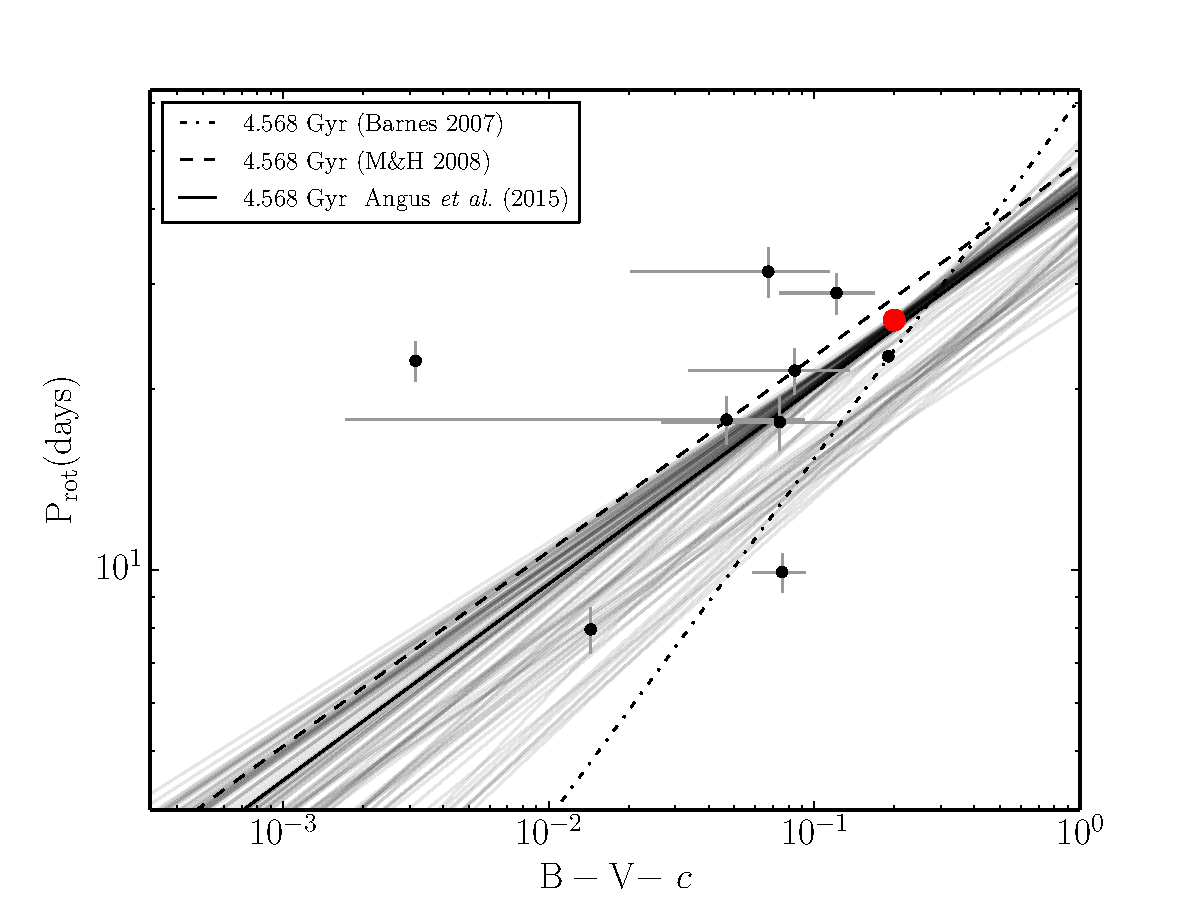
\includegraphics[width=3in, clip=true, trim=0 0 0.5in 0]{/Users/angusr/Python/Gyro/plots/p_vs_bv_solar.png}
\caption{Rotation period vs B-V colour for stars with age within 1$\sigma$ of the Sun's age, 4.568 Gyr. The grey stars are hotter than 6250 K and therefore did not contribute to the fitting process.}
\label{fig:p_vs_bv_solar}
\end{center}
\end{figure}

\begin{figure}[ht]
\begin{center}
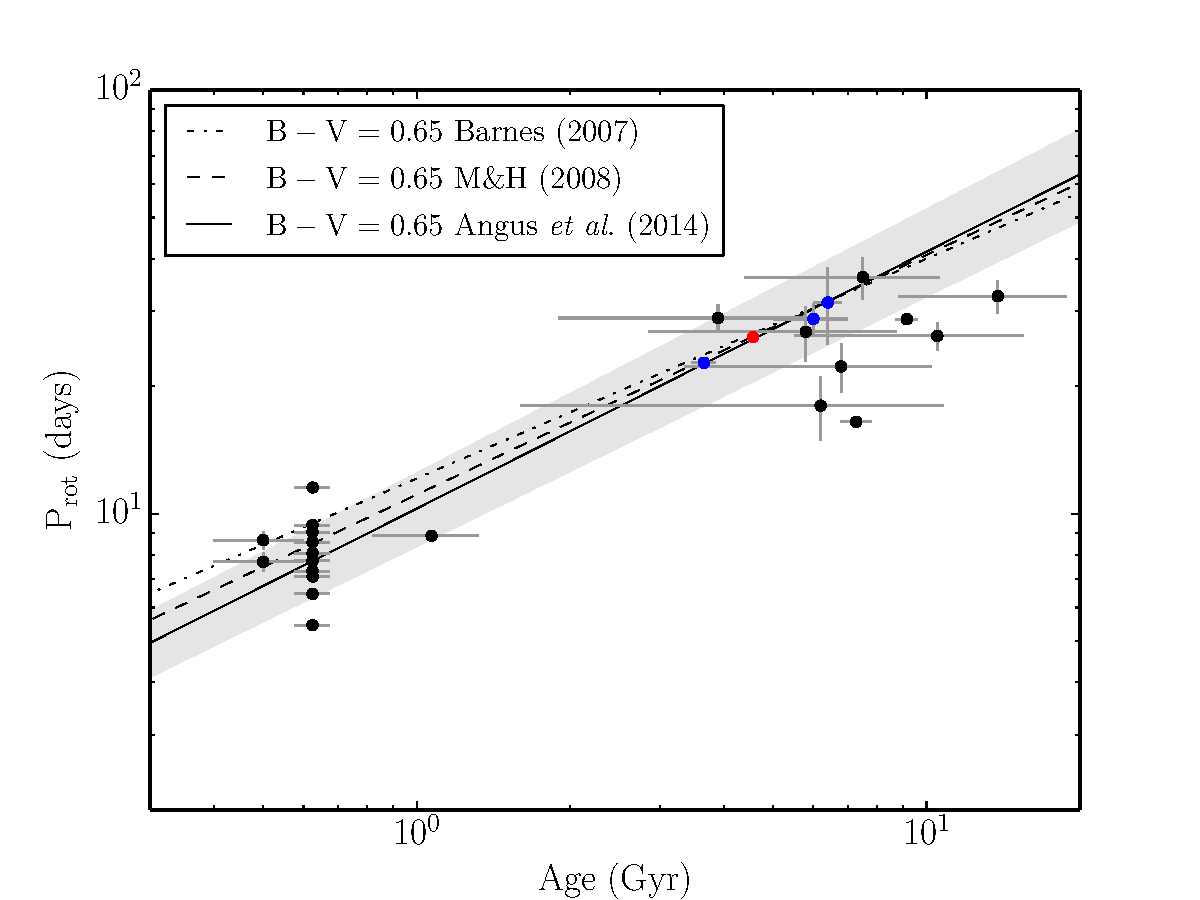
\includegraphics[width=3in, clip=true, trim=0 0 0.5in 0]{/Users/angusr/Python/Gyro/plots/p_vs_a_solar.png}
\caption{Rotation period vs age for stars with colour within 1$\sigma$ of the Sun's, 0.65.}
\label{fig:p_vs_a_solar}
\end{center}
\end{figure}

\section{Discussion}
\label{sec:discussion}

There are several possible reasons for the differences between previous and newly calibrated relations.
The first, and most obvious, is simply that the Sun is not a typical rotator for its age - it is slowly rotating.
Since previous calibrations draw their age dependence almost exlusively from the Sun, ages calculated using these gyro relations would therefore be too young.
Another explanation could be that the asteroseismic ages are systematically too old; this would make the Sun appear to be slowly rotating for its age.

Core-envelope decoupling.

The implications of a non-narrow relationship.
A relation that provides a prediction of the age of a star, given observations of \teff or colour and rotation period is the goal of gyrochronology.
The `narrowness' of the gyrochronology relation has hitherto been an unknown; do the three properties, age, mass and rotation period truely lie on an infinitely narrow plane?
Does age truely depend solely on rotation period and mass, or are there other variables that influence stellar spin down --- perhaps variables that only become important after many Myrs?
Metallicity, for example, could play a role --- a future study might explore the influence of metallicity on angular momentum loss rate.
Unfortunately, we cannot answer these questions here: the asteroseismic ages are noisy and we have not attempted to disentangle observational noise from intrinsic scatter.
A future study might include an extra parameter that describes the `width' of the gyrochronological plane.

A rift exists between theory and observation in the field of gyrochronology.
Attempts to unite theory and observation are being conducted (see, e.g. (CITATION)).

% \section{Appendix}
%
% \subsection{Probability theory}
%
% For the low-mass MS stars the joint probability can be factorised as:
%
% \begin{equation}
%   p(\hat{A}_n,\hat{P}_n,\hat{T}_n,A_n,P_n,T_n,G_n|\theta) =
%   p(A_n,P_n,T_n,G_n|\theta) p(\hat{A}_n|A_n)
%   p(\hat{P}_n|P_n) p(\hat{T}_n|T_n) p(\hat{G}_n|G_n),
% \label{eq:jointprob}
% \end{equation}
%
% \begin{equation}
% 	\propto p(A_n|P_n,T_n,G_n,\theta) p(\hat{A}_n|A_n)
% 	p(\hat{P}_n|P_n)p(P_n) p(\hat{T}_n|T_n)p(T_n) p(\hat{G}_n|G_n)p(G_n) dA_n dP_n dT_n dG_n
% \label{eq:jointprob}
% \end{equation}
%
% and the marginalised likelihood for a single star can be written as the sum of the individual star likelihoods over the three different regimes, k:
%
% \begin{multline}
% p(\hat{P}_n,\hat{A}_n,\hat{T}_n,\hat{G}_n|\theta,T_K)  = \\
% \sum_{k=1}^3\int p(A_n,T_n,P_n,G_n|\theta,T_K)
% p(\hat{A}_n|A_n) p(\hat{T}_n|T_n) p(\hat{P}_n|P_n) p(\hat{G}_n|G_n)
% {\rm d}A_n {\rm d}T_n {\rm d}P_n {\rm d}G_n,
% \end{multline}
% \label{eq:L1}
%
% where $p(A_n,T_n,P_n,G_n|\theta,T_K)$ is different in the three regimes, as listed in table \ref{tab:jprob}.

% \begin{deluxetable}{lc}
% \label{tab:jprob}
% \tablewidth{0pc}
% \tablecaption{Probability of hidden variables for the three populations.}
% \tablehead{
% \colhead{Regime}&
% \colhead{Joint probability distribution}}
% \startdata
% Low mass, MS & $p(A_n,P_n,T_n,G_n|\theta) = p_1(T_n|T_K) p_1(G_n) p_1(P_n) p(A_n|T_n,P_n,\theta)$ \\
% High mass, MS & $p(A_n,P_n,T_n,G_n|Y, V) = p(P_n) p(T_n) p(G_n) p(A_n|Y, V)$  \\
% Subgiants & $p(A_n,P_n,T_n,G_n|Z, U) = p(T_n) p(G_n) p(P_n) p(A_n|Z, U)$ \\
% \enddata
% \end{deluxetable}

% We would like to thank Eric Mamajek for his helpful input.

\bibliographystyle{plainnat}
\bibliography{Gyro_paper}

\begin{figure}[ht]
\begin{center}
\includegraphics[width=6in, clip=true, trim=0 0 0.5in 0]{/Users/angusr/angusr/ACF/ACF2/PDCQ3_output/plots_acf/3223000_full.png}
\caption{PDC-MAP and 'processed' light curves for KIC 3223000 with the ACF.}
\label{fig:lc}
\end{center}
\end{figure}

\begin{figure}[ht]
\begin{center}
\includegraphics[width=6in, clip=true, trim=0 0 0.5in 0]{/Users/angusr/angusr/ACF/ind_qs_figs/3223000.pdf}
\caption{Period measurements for quarters 3 - 16 of star `KIC 7771282'. The blue solid line indicates the median value and the shaded blue region marks its 15\% margin. The blue dashed line with surrounding shaded area indicates one half of the median period measurement with 15\% margin.  More than two thirds of the period measurements were present and consistent to within 15\% of the median for this star, so it passed the selection process.}
\label{fig:ind_qs}
\end{center}
\end{figure}

\end{document}

